\documentclass{report}
\usepackage[utf8]{inputenc}
\usepackage{graphicx}
\usepackage{multirow}
\usepackage{caption}
\usepackage{subcaption}
\usepackage{amsfonts,amssymb,amsmath}
\usepackage{multicol}
\usepackage{listings}
\usepackage{enumitem}
\lstset{
  basicstyle=\ttfamily,
  mathescape
}
\usepackage[utf8]{inputenc}
\usepackage[spanish]{babel}
\usepackage{lscape}
\usepackage[left=1.5cm,right=1.5cm,top=2cm,bottom=2cm]{geometry}

\begin{document}

\begin{center}
    
    \begin{tabular}{l c r}
    
\includegraphics[scale=0.15]{Imagenes/IPN.jpeg}
    & 
        \bf\fontsize{22}{0}{\selectfont{Instituto Polit\'ecnico Nacional}}

    
    & 
\includegraphics[scale=0.08]{Imagenes/escom.png} \\
     
    & \bf\fontsize{22}{0}{\selectfont{ Escuela Superior de C\'omputo}} &  \\
    \end{tabular}

	
	\vspace*{2\baselineskip}
	
	{
		\bf\fontsize{12}{0}{\selectfont{An\'alisis de Algoritmos, Sem: 2021-1, 3CV1, Pr\'actica 5, 8/12/20}}
	}
			
	\vspace*{2\baselineskip}
			 
	{
		\fontsize{23}{0}{\selectfont{Práctica 5: Algoritmos greedy}}
	}
	
	\vspace*{2\baselineskip}
	
	{
		\bf\fontsize{12}{0}{\selectfont{Valle Mart\'inez Luis Eduardo, Rivero Ronquillo Omar Imanol}}
	}
	
	\vspace*{1\baselineskip}
	
	{
		\fontsize{12}{0}{\textit{lvalle212@gmail.com, imanol.rivero7@gmail.com}}
	}
	
	\vspace*{2\baselineskip}

    {
	    \fontsize{12}{0}\selectfont{
	    \textbf{Resumen:} En el actual documento se presenta el análisis de algoritmos que operan bajo la estrategia de búsqueda voraz o también llamados \textbf{Greedy}}
	    
	    \fontsize{12}{0}\selectfont{
	    \textbf{Palabras Clave:} Greedy, , Java}
	
	}
\end{center}

\hfill \break
\hfill \break
\hfill \break

\chapter*{Introducción} 
    Para la creación de un algoritmo existen distintos métodos y enfoques ahora ya bastante bien conocidos y estudiados, tales como los secuenciales, los recursivos, los Greedy o voraces, etc. Y además de los anteriores aquellos que nos encontramos analizando en esta práctica, los que implementan la programación dinámica mediante el uso de memoización, en la mayoria de los casos. Sin embargo, para hacer uso de estos enfoques nuestro problema deberá cumplir con ciertas condiciones, que más adelante serán mencionadas.

Como podemos ver, se cuenta con una amplia gama de técnicas y muy probablemente no sea tan sencillo escoger entre ellas, pero finalmente es tarea de la ingeniería conocer todos estas técnicas y enfoques para finalmente elegir cúal es el que hace mejor se adapta a la problematica que se busca resolver.

Los algoritmos que se analizan y prueban en este documento son algoritmos clásicos bien estudiados por todos aquellos profesionales pertenecientes a las ciencias de la computación, pero esta reputación de clásicos, no se debe solamente a que ejemplifican perfectamente el uso de los métodos con las que son implementadas, pero por que son simplemente útiles para la resolución de problemáticas con las que cotidianamente lidian, tanto profesionales como no expertos en el área donde surge la necesidad de encontrar solución a una situación.

Siendo una de las sucesiones de números más fascinantes que encontramos directamente describiendo fenómenos de la naturaleza con Fibonacci. O el amplio abanico de problemas en los que puede implementarse, mediante variaciones del problema original, la Mochila entera para encontrar la solución a problemas específicos de un área.

\chapter*{Conceptos B\'asicos}
   \section*{Divide y vencerás}
    El nacimiento de esta frase se remonta al gran Julio César, prestigioso militar y político romano nacido en los años 100 a.C., teniendo su origen en el hecho de que los romanos al conquistar un territorio, se abstenían de oprimir a los vencidos, evitando rebeliones y la formación de un frente común. Para evitar esto, además los romanos firmaban contratos con cada pueblo de manera individual, otorgando derechos distintos y de número irregular a cada uno, provocando envidias entre los mismos pueblos, y por consiguiente imposibilitando la unión.\\
    
    Con el pasar del tiempo, se convirtió en un refrán popular que implica resolver un problema difícil, dividíendolo en partes más simples tantas veces como sea necesario, hasta que la solución de las partes sea obvia, de esta forma la solución del problema principal se construye con las soluciones encontradas.\\
    
    De esta forma llegó hasta las ciencias de la computación, convirtiéndose en uno de los paradigmas más importantes en el diseño algorítmico. Esta basado en la resolución recursiva de un problema que se divide un subproblemas del mismo tipo hasta que resulten lo suficientemente sencillos para realizar de forma directa. El resultado final entonces, se conforma de la combinación  de los resultados de los subproblemas, dando una solución final al problema general.\\
    
    De esta técnica se tienen algoritmos muy eficientes para la resolución de cualquier tipo de problema, ejemplos basados en esta técnica se tiene:\\
    \begin{itemize}
        \item Algoritmo de Ordenamiento: QuickSort, MergeSort
        \item Multiplicar números grandes: Karatsuba
        \item Análisis sintáctico: análisis sintáctico top-down
        \item Transformada discreta de Fourier
    \end{itemize}
    
\section*{Algoritmos de ordenamiento}
    Los algoritmos de ordenamiento son algoritmos que colocan los elementos de un array, lista o vector, en una secuencia específica descrita por una relación de orden.\\
    
    Los órdenes más comunes son el numérico y lexicográfico, siendo el último una relación de orden definida sobre el producto cartesiano de conjuntos ordenados. Es principalmente concido por la aplicación a cadenas de caracteres en diccionarios, guias telefónicas, etc.\\
    
    La salida de estos algoritmos deben de satisfacer 2 condiciones:
    \begin{enumerate}
        \item La salida debe de encontrarse en orden no-decreciente
        \item La salida es una permutación o re-ordenamiento de la entrada
    \end{enumerate}
    
    Hay métodos muy simples de implementar que son útiles en los casos en dónde el número de elementos a ordenar no es muy grande. Pero por otro lado hay métodos sofisticados, más difíciles de implementar pero que son más eficientes en cuestión de tiempo de ejecución.
    
    Los métodos sencillos por lo general requieren de aproximadamente n x n pasos para ordenar n elementos.
    
    Los métodos simples con complejidad cuadrática son:
    \begin{itemize}
        \item Insertion Sort
        \item Selection Sort
        \item Bubble Sort
        \item Shell Sort(extensión más veloz del bubble sort)
    \end{itemize}
    
    Los métodos más complejos acortan el tiempo de ejecución y por lo tanto son más eficiente:
    \begin{itemize}
        \item Quick Sort
        \item Merge Sort
        \item Heap Sort
        \item Radix
        \item Address-calculation Sort
    \end{itemize}
    
    Existen diferentes maneras de clasificar los algoritmos de ordenamiento:
    
    \textbf{Clasificación según el lugar donde se realiza la ordenación}\\
    \begin{itemize}
        \item Ordenamiento interno: Se realiza el ordenamiento enteramente en la memoria primaria del ordenador
        \item Ordenamiento externo: Aquellos que involucran discos auxiliares para guardar resultados intermedios
    \end{itemize}
    
    \textbf{Clasificación por el tiempo que tardan en la ordenación}\\
    \begin{itemize}
        \item Ordenación natural: Tarda lo mínimo posible con la entrada ordenada
        \item Ordenación no natural: Tarda lo mínimo posible cuando la entrada esta inversamente ordenada 
    \end{itemize}
    
    \textbf{Por estabilidad}\\
    En un ordenamiento estable se mantiene el orden relativo que tenian originalmente los elementos con claves iguales. Esto es, con un algoritmo estable habrá 2 registros R y S con la misma clave y con R apareciendo antes que S en la lista original.\\
    
    En elementos que son indistiguibles entre si, la estabilidad no es un problema, tal y como sucede con los números enteros, pero en general se puede decir que se despecia la estabilidad cuando el elemento entero es la clave.\\
    
\section*{Merge Sort}
    Merge Sort es un algoritmo desarrollado con la técnica de divide y vencerás, creado por Jhon Von Newmann en 1945. De propósito general, es un algoritmo que produce un ordenamiento estable con complejidad O(nlogn). Utiliza memoria auxiliar con complejidad O(n), dado por el algoritmo \textit{Merge}.\\
    
    La familia de algoritmos \textit{Merge}, toman una multiple lista ordenada como entrada y produce una lista única ordenada como salida, conteniendo todos los elementos de la lista de entrada. Estos algoritmos son utilizados como subrutinas para varios algoritmos de ordenamiento, siendo el más famoso precisamente \textit{Merge Sort}.\\
    
    \textit{Merge Sort} inicia con la entrada de un arreglo, este divide el arreglo de entrada en 2 mitades, se llama a si mismo para las 2 mitades y después mezcla las mitades con ayuda del algoritmo \textit{Merge}.\\
    
    Gráficamente la operación del algoritmo se muestra en la siguiente figura \ref{OperacionMergeSort}:
    \begin{figure}[h!]
        \centering
        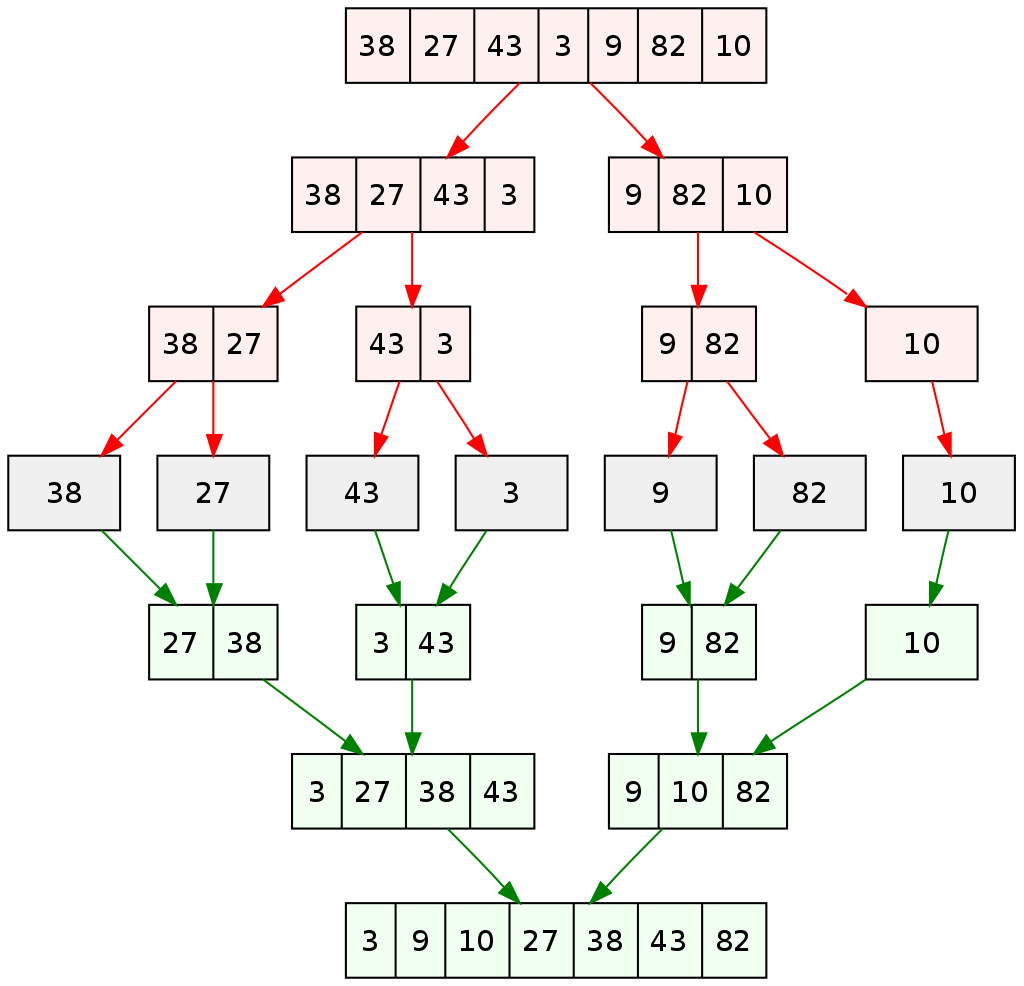
\includegraphics[width=10cm]{OperacionMergeSort.png}
        \caption{Ordenamiento de un arreglo de 7 valores enteros utilizando el algoritmo \textit{MergeSort}}
        \label{OperacionMergeSort}
    \end{figure}
    
\section*{Quick Sort}
    Quick Sort es un algoritmo basado en la técnica divide y vencerás creado por el científico británico C. A. R. Hoare, quién también es conocido como Tony Hoare, en el año de 1960.\\
    
    Es el algoritmo más ampliamente utilizado en el mundo para el ordenamiento numérico, también es considerado el algoritmo más eficiente y veloz de los métodos de ordenación interna.
    
    La complejidad del algoritmo para su caso promedio es O(nlogn), pero en su peor caso tendrá la complejidad O($n^2$), dandose este caso cuando el pivote queda en alguno de los extremos.
    
    El funcionamiento del algoritmo se describe en 4 pasos:\\
    \begin{enumerate}
        \item Se elige un elemento de la lista a ordenar, se le llamará pivote
        \item Se reacomodan los elementos de la lista según el valor de pivote, de manera que los elementos antes de este son siempre menores, y los que están después serán siempre mayores. Después de este ordenamiento parcial, el pivote ya se encuentra colocado en el lugar exacto que debe ocupar en la lista final.
        \item La lista se separa en 2 sublistas, una formada por los elementos a la izquierda del pivote, y otra por los elementos a su derecha.
        \item Se repite el proceso de forma recursiva para todas las sublistas mientras estas contengan más de un elemento. Al terminar este proceso todos los elemento se encuentran ordenados.
    \end{enumerate}
    
    En este algoritmo la elección del pivote es muy importante, pues dependiendo de la elección, el algoritmo puede ser más o menos eficiente. Si bien tomar un elemento cualquiera como pivote no requiere de cálculo alguno, la elección a ciegas puede provocar para ciertas entradas una complejidad de O($n^2$).\\
    
    Una alternativa para subsanar este problema es conocer de antemano el elemento central para utilizar como pivote, esta operación puede realizarse en O(n) y asegura hasta para el peor de los casos que el algoritmo sea O(nlogn), sin embargo este cálculo adicional rebaja la eficiencia en el caso promedio.\\
    
    Otra opción es tomar tres elementos de la lista, comúnmente se escoge el primero, medio y último elemento del arreglo, se comparan y el valor medio es escogido como el pivote.

\chapter*{Experimentación y Resultados}
        \section*{Códigos de Huffman}
        \hfill \break

\subsection*{Análisis a priori}

    Consideremos el pseudocódigo descrito en la figura \ref{PseudocodigoHuffman} para la codificacion de Huffman.

    \begin{figure}[h!]
        \centering
        \begin{verbatim}
            Huffman(C: arreglo de caracteres sin repeticion)
                n = |C|
                Q = cola_prioridad(C)
                for i=1 to i<=n do
                    x = Q.extraerMin()
                    y = Q.extraerMin()
                    z = nuevo_nodo
                    z.izq = x
                    z.der = y
                    z.frec = x.frec + y.frec
                    Q.insertar(z)
                return Q
        \end{verbatim}  
        \caption{Pseudocódigo del algoritmo de la codificacion de Huffman}
        \label{PseudocodigoHuffman}
    \end{figure}
    
    Podemos observar en la figura \ref{PseudocodigoHuffman} que el algoritmo hace uso de una cola de prioridad, llamada Q para sacar los nodos con la menor frecuencia en cada iteración. Posteriormente se crea un nuevo nodo que tiene como hoja izquierda al nodo con la menor frecuencia de los dos y como hoja derecha al que tiene una mayor frecuencia. A continuación se calcula la complejidad del algoritmo por análisis por bloque.
    
    \begin{equation*}
        \left.
            \begin{aligned}
                \left.
                    \begin{aligned}
                        \text{n = C.size} \\
                        \text{Q = colaprioridad(C)}
                    \end{aligned}
                \right\}
                \quad\Theta(1)
                \\
                \left.
                    \begin{aligned}
                        \text{for i=1 to i<=n do} \\
                        \left.
                            \begin{aligned}
                                \text{x = Q.extraerMin()} \\
                            \end{aligned}
                        \right\}
                        \quad\Theta(log(n))
                        \\
                        \left.
                            \begin{aligned}
                                \text{y = Q.extraerMin()} \\
                            \end{aligned}
                        \right\}
                        \quad\Theta(log(n))
                        \\
                        \left.
                            \begin{aligned}
                                \text{z = nuevonodo} \\
                                \text{z.izq = x} \\
                                \text{z.der = y} \\
                                \text{z.frec = x.frec + y.frec} \\
                            \end{aligned}
                        \right\}
                        \quad\Theta(log(n))
                        \\
                        \left.
                            \begin{aligned}
                                \text{Q.insertar(z)} \\
                            \end{aligned}
                        \right\}
                        \quad\Theta(log(n))
                        \\
                        \text{return Q} \\
                    \end{aligned}
                \right\}
                \quad\Theta(nlog(n))
            \end{aligned}
        \right\}
        \quad\Theta(nlog(n))
    \end{equation*}
    
    Finalmente, la complejidad del algoritmo de la codificacion de Huffman esta dado por $\Theta(nlog(n))$. Es interesante observar que usar las operaciones de extraer e insertar son las que agregan la complejidad logaritmica $\Theta(log(n))$ debido a la forma en la que insertan y extraen elementos de su heap, siendo el heap también un arbol que describe la prioridad de sus elementos. 

\subsection*{Análisis a posteriori}

    Para la generación de nuestras gráficas, se realizó un conteo del número de operaciones realizadas en el algoritmo para cada arreglo de tamaño n de caracteres sin repeticion. Se utilizaron archivos de texto que se trabajan para generar su codifcación de Huffman, su árbol asociado y su decodificacion final. Los archivos se construyeron considerando los caracteres que iban a contener quitando sus repeticiones. Por ejemplo:
    
    Teniendo como entrada un archivo que contuviera la cadena "bbbaaaccfffttat", nuestro arreglo sin repeticiones seria [b,a,c,f,t] y la n asociada sería n=5.
    
    En la figura \ref{GraficaHuffman} se presenta la gráfica generada por nuestra implementación.
    
    \begin{figure}[h!]
        \centering
        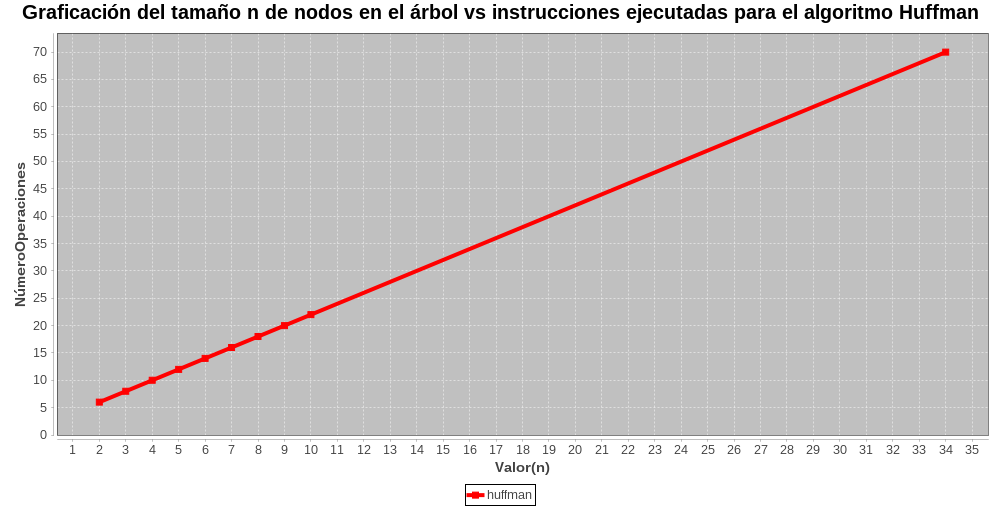
\includegraphics[width=13cm]{Huffman/graf-huffman.png}
        \caption{Representación gráfica de la complejidad temporal del algoritmo de la codificación de Huffman, mediante la evaluación del número de instrucciones realizadas.}
        \label{GraficaHuffman}
    \end{figure}
    
    Teniendo como puntos al siguiente arreglo, mostrado en la figura \ref{PuntosHuffman}:
    
    \begin{figure}[h!]
        \centering
        \begin{tabular}{c|c}
            P1( 2,6 ) & P5( 6,14 )\\
            P2( 3,8 ) & P6( 7,16 )\\
            P3( 4,10 ) & P7( 8,18 )\\
            P4( 5,12 ) & P8( 9,20 )\\
            P10( 10,22 ) & P11( 34, 70)
        \end{tabular}
        \caption{Pares obtenidos de la evaluación del algoritmo de la codificación de Huffman}
        \label{PuntosHuffman}
    \end{figure}
    
    Como se puede notar a simple vista, el algoritmo parece tener una complejidad lineal dada por $\Theta(n)$. Sin embargo, la causa de este desvio con nuestro análisis a priori fue que no se hizo una implementación propia de una cola de prioridad con sus operaciones, si no, que se utilizó la clase PriorityQueue definida por el lenguaje Java. Por lo tanto no fue posible considerar las instrucciones ejecutadas durante cada operacion de la cola de prioridad, causando que la complejidad aparente fuera lineal cuando debería ser $\Theta(nlog(n))$. A continuación en la figura , se representan los puntos en un graficador con la ecuación que los delimita $y=2x+2$ y la ecuación por la que deberían de estar acotados $y=xlog(x)$.
    
    \begin{figure}[h!]
        \centering
        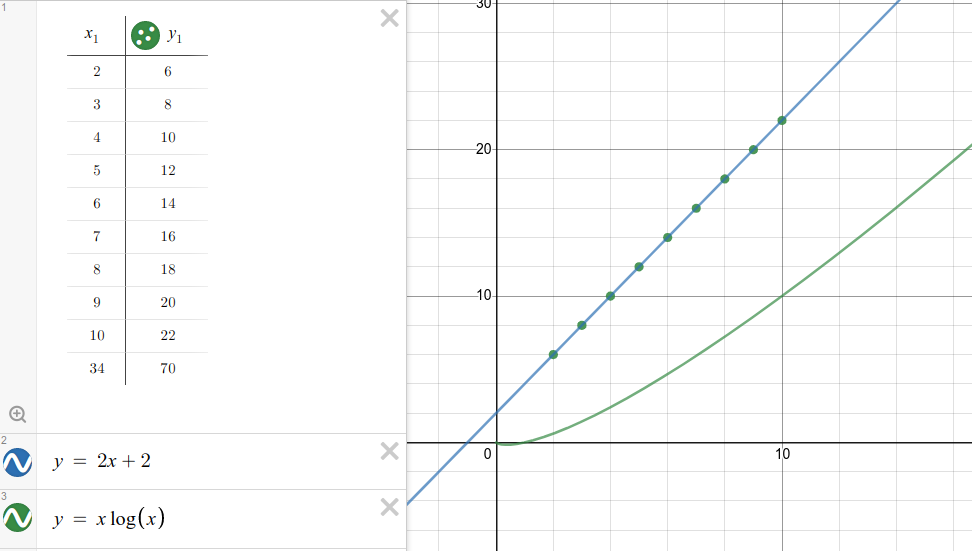
\includegraphics[width=13cm]{Huffman/graf-desm-huffman.png}
        \caption{Representación gráfica de la complejidad temporal del algoritmo de la codificación de Huffman, comparado con la ecuacion que los delimita en color azul $y=2x+2$ y la ecuación por la que deberian de estar acotados $y=xlog(x)$}
        \label{GraficaHuffman}
    \end{figure}
    \newpage
    
\subsection*{Proceso de compresión y descompresión}
    
    Para comprimir nuestro archivo de entrada sustituimos cada caracter por su representación de la conficación de Huffman que se guarda en un diccionario, y se forma una nueva cadena con una representación binaria de la salida comprimida. \\
    
    Para descomprimir una cadena que esta en su representación de Huffman, necesitamos el arbol que contiene su representación. Se recorre el arbol y si se alcanza una de las hojas, se extrae el caracter que representa y se guarda en un string que tendrá como salida a la cadena decodificada. \\
    
    La tasa de compresión se calcula considerando que la cadena de entrada original esta codificada en utf-8, por lo que cada caracter representa un byte, es decir, 8 bits. En nuestra salida codificada, cada caracter representa un bit. Finalmente, mediante una regla de 3, siendo el 100\% el numero de bits de la cadena original, calculamos la tasa de compresión.
    
    \subsubsection{Ejemplo 1}
        \begin{itemize}
            \item \textbf{Texto de origen} \\
            Era de noche. En la vasta sala silenciosa, tenuemente alumbrada por unas luces ocultas en los muros transparentes, los cuatro terrestres, sentados alrededor de
una mesa de madera conversaban en voz baja, con los rostros juntos y pálidos.
Hombres y mujeres yacían desordenadamente por el suelo. En los rincones
oscuros había leves estremecimientos: hombres o mujeres solitarios que movían
las manos. Cada media hora uno de los terrestres intentaba abrir la puerta de
plata.
-No hay nada que hacer. Estamos encerrados.
-¿Creen realmente que somos locos, capitán?
-No hay duda. Por eso no se entusiasrnaron al vernos. Se limitaron a tolerar lo que
entre ellos debe de ser un estado frecuente de psicosis. -Señaló las formas
oscuras que yacían alrededor.-Paranoicos todos. ¡Qué bienvenida! -Una llamita se
alzó y murió en los ojos del capitán.-Por un momento creí que nos recibían como
merecíamos. Gritos, cantos y discursos. Todo estuvo muy bien, ¿no es cierto?
Mientras duró. 
            \item \textbf{Compresión} \\
                \begin{figure}[h!]
                    \centering
                    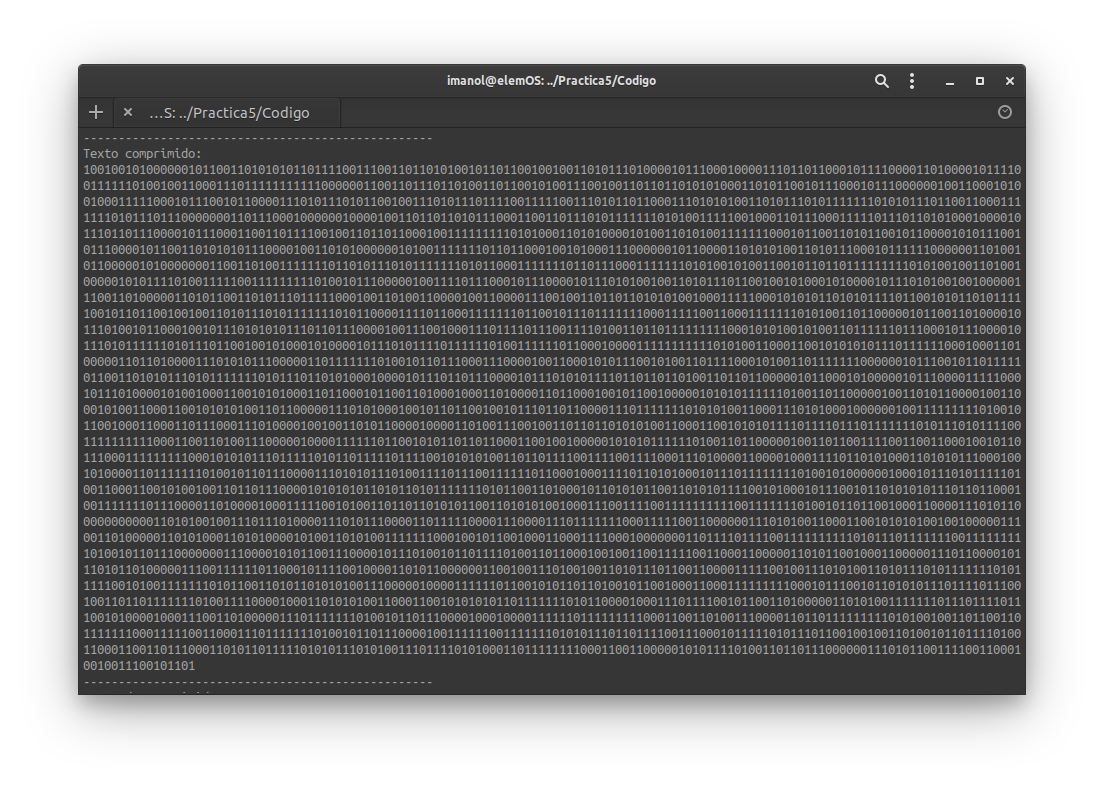
\includegraphics[width=17cm]{Huffman/ejemplos/ejemplo1/ej1-comp.png}
                \end{figure}
                \newpage
            \item \textbf{Tasa de compresión:} 54.296875\% \\
            \item \textbf{Descompresión} \\
                \begin{figure}[h!]
                    \centering
                    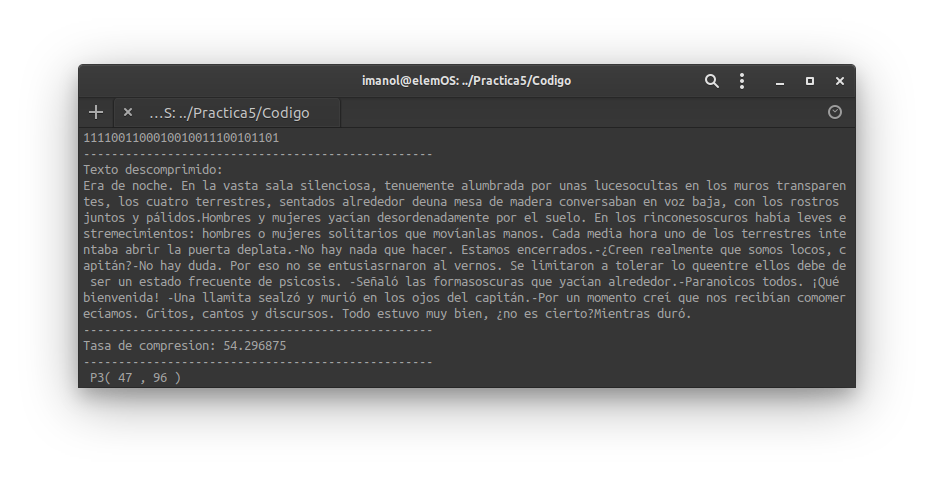
\includegraphics[width=17cm]{Huffman/ejemplos/ejemplo1/ej1-decode.png}
                \end{figure}
                \newpage
            \item \textbf{Codificación asignada} \\
                \begin{figure}[h!]
                    \centering
                    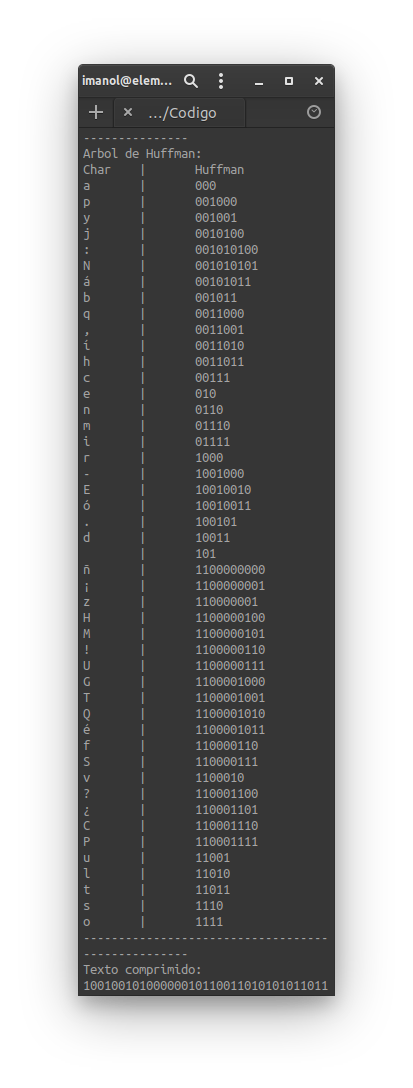
\includegraphics[scale=.5]{Huffman/ejemplos/ejemplo1/ej1-reph.png}
                \end{figure}
                \newpage
        \end{itemize}
    \subsubsection{Ejemplo 2}
        \begin{itemize}
            \item \textbf{Texto de origen} \\
            Las llamas azules brotaban alrededor de los terrestres, brillaban un momento, y se
desvanecían. Unos diablillos de arena roja corrían entre los dientes de los
hombres dormidos. Las mujeres se transformaban en serpientes aceitosas. Había
un olor de reptiles y bestias. 
            \item \textbf{Compresión} \\
                \begin{figure}[h!]
                    \centering
                    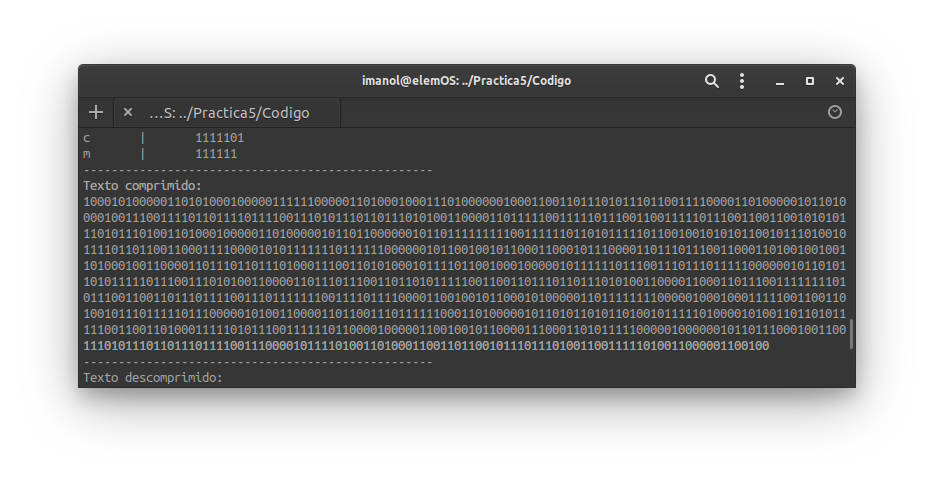
\includegraphics[width=17cm]{Huffman/ejemplos/ejemplo2/ej2-comp.png}
                \end{figure}
                \newpage
            \item \textbf{Tasa de compresión:} 51.089016\% \\
            \item \textbf{Descompresión} \\
                \begin{figure}[h!]
                    \centering
                    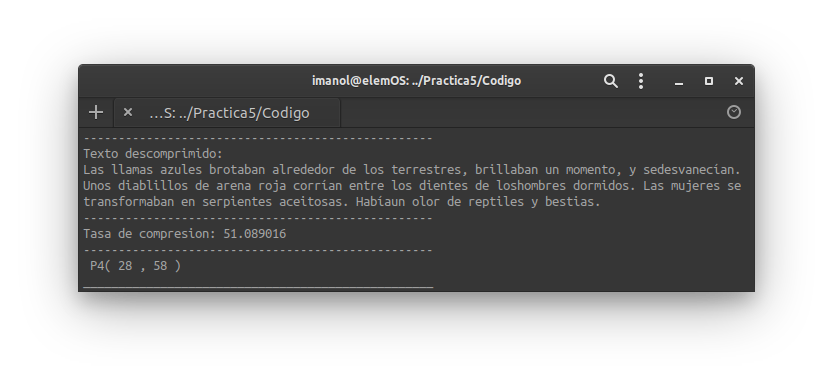
\includegraphics[width=17cm]{Huffman/ejemplos/ejemplo2/ej2-decode.png}
                \end{figure}
                \newpage
            \item \textbf{Codificación asignada} \\
                \begin{figure}[h!]
                    \centering
                    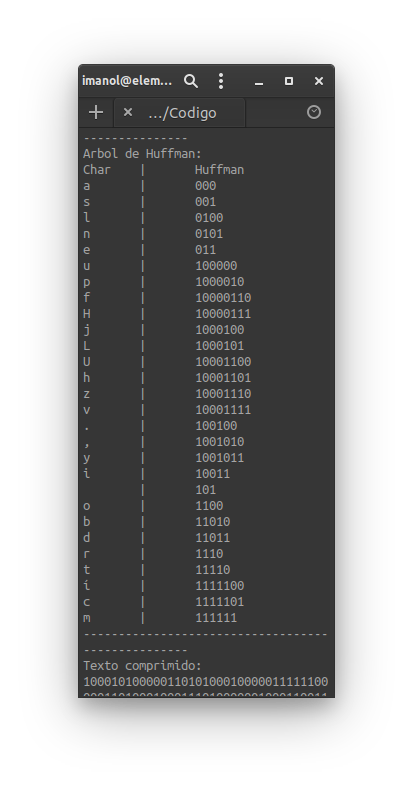
\includegraphics[scale=.5]{Huffman/ejemplos/ejemplo2/ej2-reph.png}
                \end{figure}
                \newpage
        \end{itemize}
    \subsubsection{Ejemplo 3}
        \begin{itemize}
            \item \textbf{Texto de origen} \\
            Qué demencia más hermosa. Metal, caucho, gravitadores, comida, ropa,
combustible, armas, escaleras, tuercas, cucharas. He comprobado que en su nave
hay diez mil artículos distintos. Nunca había visto tal complejidad. Hay hasta
sombras debajo de las literas y debajo de todo. ¡Qué poder de concentración! Y
todo, no importan cuándo o cómo se pruebe, tiene olor, solidez, gusto, sonido.
Permítame que lo abrace.-El psiquiatra abrazó al capitán.- Consignaré todo esto
en lo que será mi mejor monografia. El mes que viene hablaré en la Academia
Marciana. Mírese. Ha cambiado usted hasta el color de sus ojos, del amarillo al
azul, y la tez de morena a sonrosada. ¡Y su ropa, y sus manos de cinco dedos en
vez de seis! ¡Metamorfosis biológica a través del desequilibrio psicológico! Y sus
tres amigos... 
            \item \textbf{Compresión} \\
                \begin{figure}[h!]
                    \centering
                    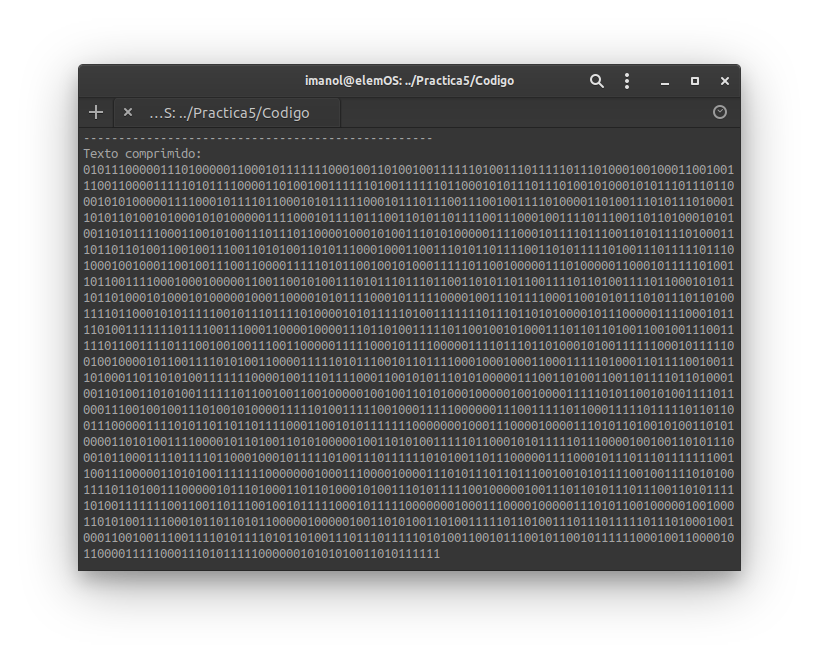
\includegraphics[width=17cm]{Huffman/ejemplos/ejemplo3/ej3-comp.png}
                \end{figure}
                \newpage
            \item \textbf{Tasa de compresión:} 56.04378\% \\
            \item \textbf{Descompresión} \\
                \begin{figure}[h!]
                    \centering
                    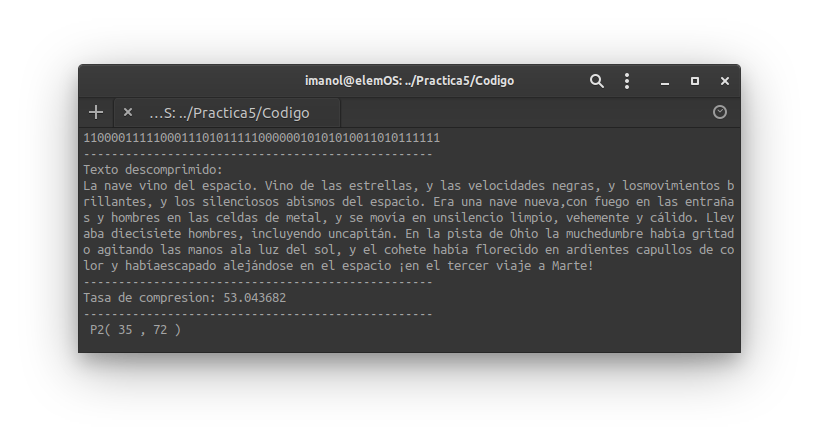
\includegraphics[width=17cm]{Huffman/ejemplos/ejemplo3/ej3-decode.png}
                \end{figure}
                \newpage
            \item \textbf{Codificación asignada} \\
                \begin{figure}[h!]
                    \centering
                    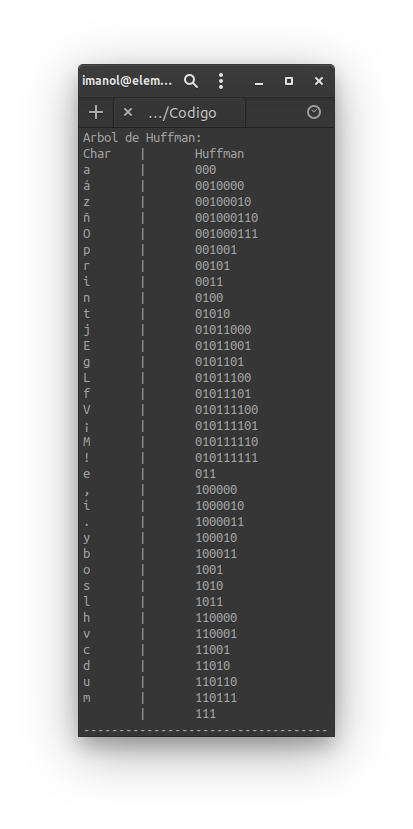
\includegraphics[scale=.5]{Huffman/ejemplos/ejemplo3/ej3-reph.png}
                \end{figure}
                \newpage
        \end{itemize}
    \subsubsection{Ejemplo 4}
        \begin{itemize}
            \item \textbf{Texto de origen} \\
            Quería ir a Marte en el cohete. Bajó a la pista en las primeras horas de la mañana
y a través de los alambres les dijo a gritos a los hombres uniformados que quería
ir a Marte. Les dijo que pagaba impuestos, que se llamaba Pritchard y que tenía el
derecho de ir a Marte. ¿No había nacido allí mismo en Ohio? ¿No era un buen
ciudadano? Entonces, ¿por qué no podía ir a Marte? Los amenazó con los puños
y les dijo que quería irse de la Tierra; todas las gentes con sentido común querían
irse de la Tierra. Antes que pasaran dos años iba a estallar una gran guerra
atómica, y él no quería estar en la Tierra en ese entonces. Él y otros miles como
él, todos los que tuvieran un poco de sentido común, se irían a Marte. Ya lo iban a 
32
ver. Escaparían de las guerras, la censura, el estatismo, el servicio militar, el
control gubernamental de esto o aquello, del arte y de la ciencia. ¡Que se
quedaran otros! Les ofrecía la mano derecha, el corazón, la cabeza, por la
oportunidad de ir a Marte. ¿Qué había que hacer, qué había que firmar, a quién
había que conocer para embarcar en un cohete?

Los hombres de uniforme se rieron de él a través de los alambres. No quería ir a
Marte, le dijeron. ¿No sabía que las dos primeras expediciones habían fracasado y
que probablemente todos sus hombres habían muerto?
            \item \textbf{Compresión} \\
                \begin{figure}[h!]
                    \centering
                    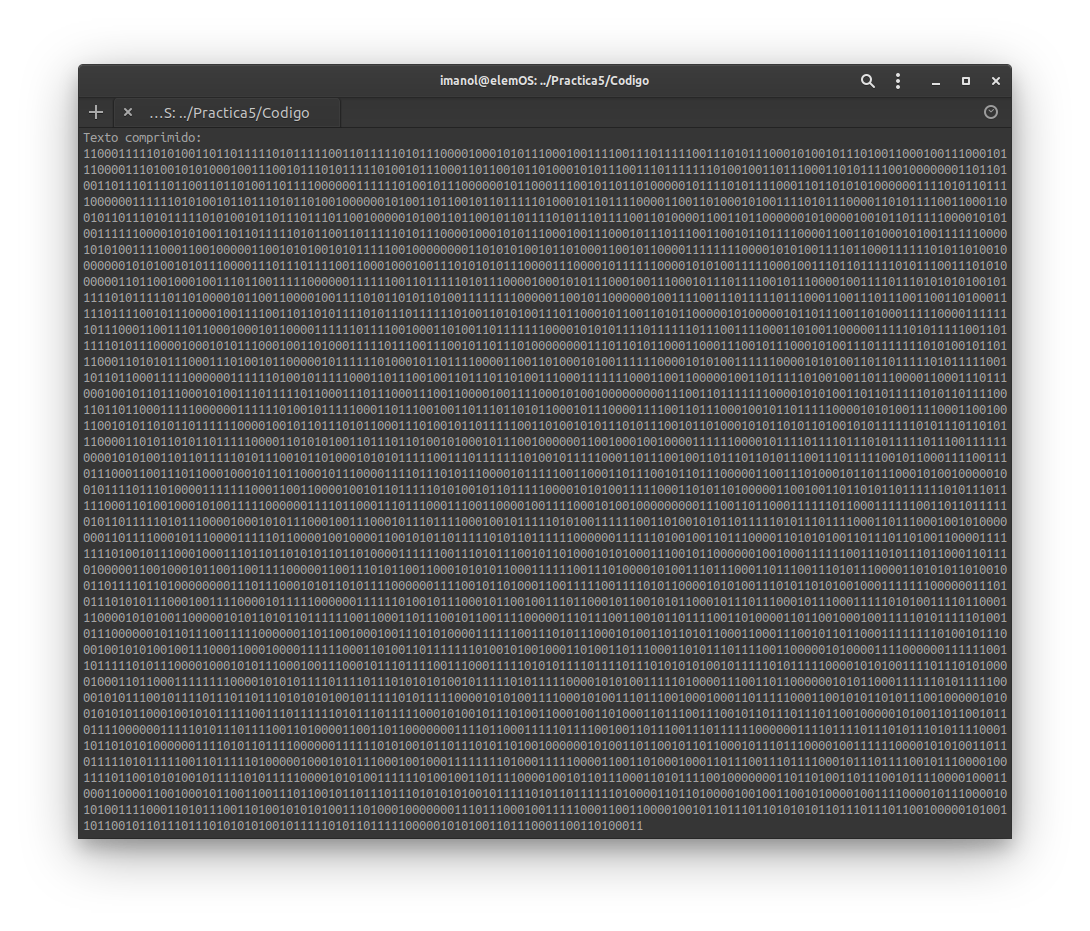
\includegraphics[width=17cm]{Huffman/ejemplos/ejemplo4/ej4-comp.png}
                \end{figure}
                \newpage
            \item \textbf{Tasa de compresión:} 54.70817\% \\
            \item \textbf{Descompresión} \\
                \begin{figure}[h!]
                    \centering
                    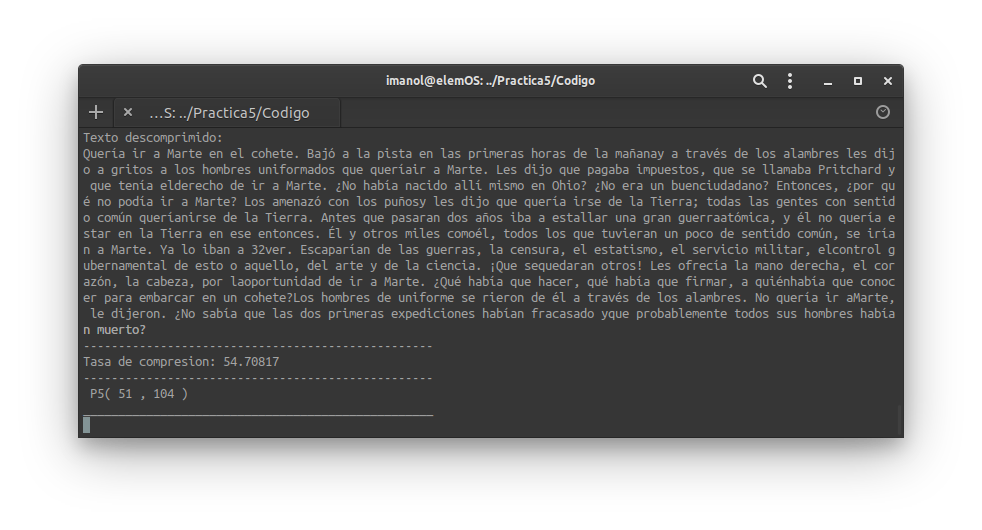
\includegraphics[width=17cm]{Huffman/ejemplos/ejemplo4/ej4-decode.png}
                \end{figure}
                \newpage
            \item \textbf{Codificación asignada} \\
                \begin{figure}[h!]
                    \centering
                    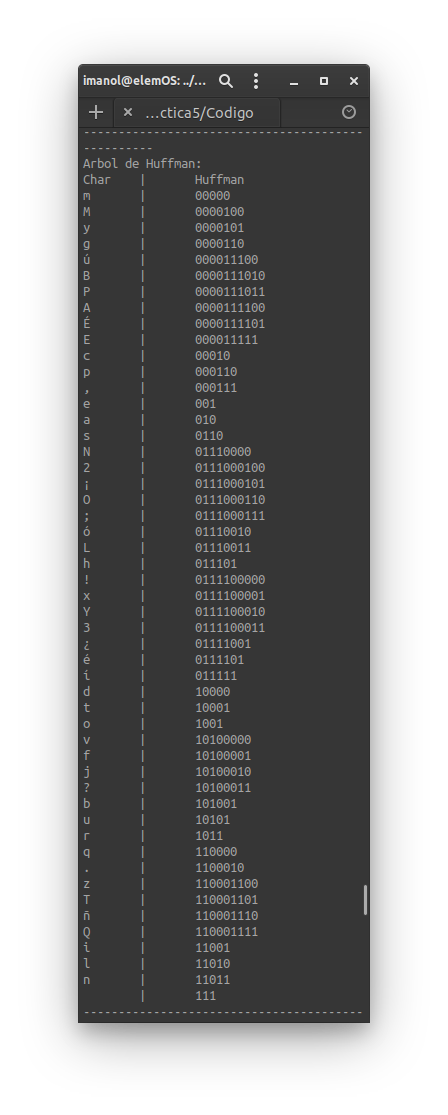
\includegraphics[scale=.5]{Huffman/ejemplos/ejemplo4/ej4-reph.png}
                \end{figure}
                \newpage
        \end{itemize}
    \subsubsection{Ejemplo 5}
        \begin{itemize}
            \item \textbf{Texto de origen} \\
            La nave vino del espacio. Vino de las estrellas, y las velocidades negras, y los
movimientos brillantes, y los silenciosos abismos del espacio. Era una nave nueva,
con fuego en las entrañas y hombres en las celdas de metal, y se movía en un
silencio limpio, vehemente y cálido. Llevaba diecisiete hombres, incluyendo un
capitán. En la pista de Ohio la muchedumbre había gritado agitando las manos a
la luz del sol, y el cohete había florecido en ardientes capullos de color y había
escapado alejándose en el espacio ¡en el tercer viaje a Marte! 
            \item \textbf{Compresión} \\
                \begin{figure}[h!]
                    \centering
                    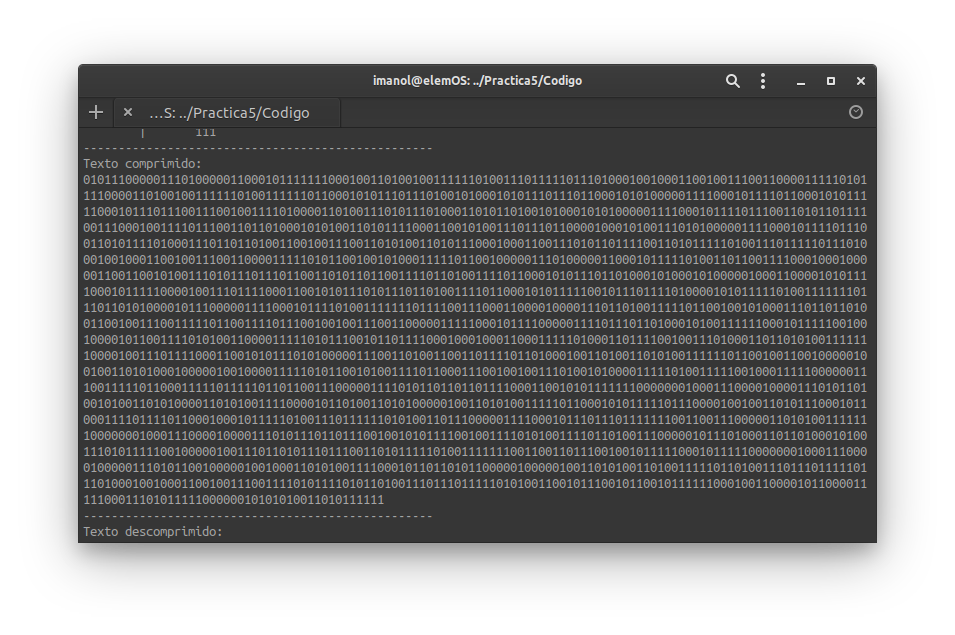
\includegraphics[width=17cm]{Huffman/ejemplos/ejemplo5/ej5-comp.png}
                \end{figure}
                \newpage
            \item \textbf{Tasa de compresión:} 53.043682\% \\
            \item \textbf{Descompresión} \\
                \begin{figure}[h!]
                    \centering
                    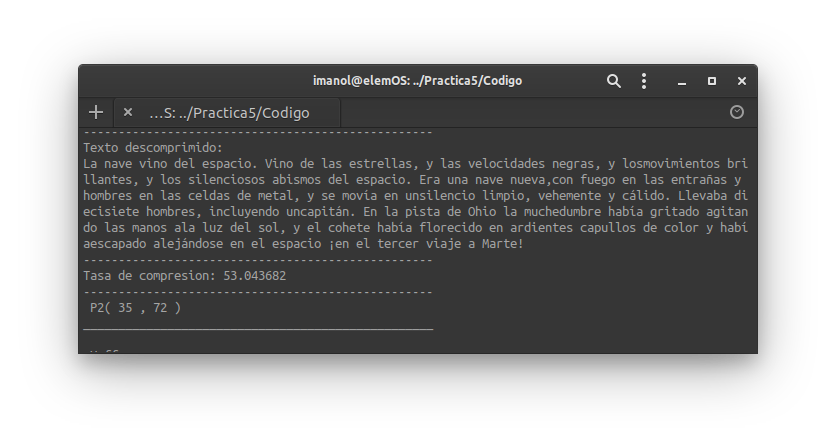
\includegraphics[width=17cm]{Huffman/ejemplos/ejemplo5/ej5-decode.png}
                \end{figure}
                \newpage
            \item \textbf{Codificación asignada} \\
                \begin{figure}[h!]
                    \centering
                    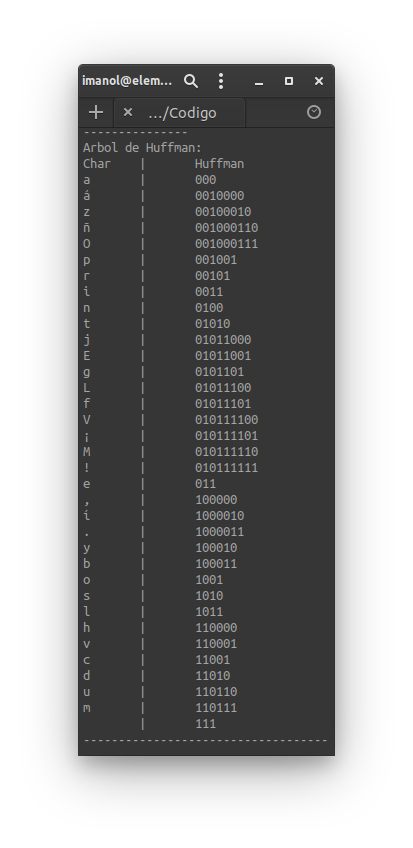
\includegraphics[scale=.5]{Huffman/ejemplos/ejemplo5/ej5-reph.png}
                \end{figure}
                \newpage
        \end{itemize}
        \newpage
    
    \section*{Algoritmo de Kruskal}
        \subsection*{Aplicaciones del Algoritmo de Kruskal}

    Existen diversas aplicaciones del algoritmo en un escenario real mediante la industria.\\
    
    Los problemas más socorridos por este algoritmo son aquellos que tienen que ver con distancias y puntos fijos en un área geográfica. De esta forma el problema de la distribución de los cables a las tomas o estaciones fijas repartidas en la ciudad, a cargo empresas del sector de las telecomunicaciones y servicios eléctricos, se auxilian de este para identificar el cableado más corto y conecte a un número de nodos fijos, significa menores costos en muchos de los aspectos insfraestructurales.
    
    Así mismo, puede ser considerada una problemática similar la ruta que conecta estaciones perteneciente a algún servicio de transporte, tal como un Metro, Tren o similares. Este algoritmo les auxilia permientiendo no solo disminuir costos para la construcción, y mantenimiento, pero asegura la ruta que más rápidamente permite el transporte de los usuarios, significando un ahorro también en el tiempo.

\subsection*{Análisis a posteriori}
    Para obtener una gráfica descriptiva y que permitiera realizar un análisis mediante una aproximación de forma correcta, se decidió que se evaluarián, al menos, grafos con un número total de 10 nodos o aristas.
    
    Para la descripción de los grafos, se utilizaron archivos donde cada fila corresponde a la descripción de un nodo. La sintaxis para la descripción del nodo inicia con el nombre del nodo, se colocan entre llaves los pares que corresponden a las trasiciones con otros nodos y el costo de la arista separando cada par por comas, de forma que se coloca primero el nombre del nodo destino y seguido de un signo de \$ el costo del vértice. Un ejemplo de la descripción de un grafo sería la siguiente \ref{GrafoEjemplo}:
    \begin{figure}[h!]
        \centering
        \begin{verbatim}
            Nodo1{ Nodo2$5 , Nodo3$12}
            Nodo2{ Nodo1$1 }
            Nodo3{ Nodo1$6 , Nodo2$8}\end{verbatim}
        \caption{Ejemplo de grafo descrito en el archivo ingresado al programa}
        \label{GrafoEjemplo}
    \end{figure}
    
    Los resultados obtenidos por el programa se muestran iniciando con \textbf{F}, le procede un signo de \$ y un número entero, que indica el coste total de árbol encontrado, y finalmente entre llaves se colocan los pares de nodos que conforman a este árbol mínimo \ref{ResultadoEjemplo}:
    
    \begin{figure}[h!]
        \centering
        \begin{verbatim}
            F$7 = {(Nodo2,Nodo1) (Nodo3,Nodo1)}\end{verbatim}
        \caption{Ejemplo de los elementos que conforman los resultados obtenidos del programa}
        \label{ResultadoEjemplo}
    \end{figure}
    
    A continuación se muestran los grafos evaluados:
    
    \subsubsection*{Grafo de 3 nodos}
        Grafo muy sencillo de únicamente 3 nodos. Fig\ref{Grafo3} y su estructura en \ref{ArchivoGrafo3}.
        
        \begin{figure}[h!]
            \centering
            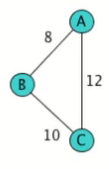
\includegraphics{Kruskal/Grafo3.png}
            \caption{Gráfo de 3 nodos y 3 arcos}
            \label{Grafo3}
        \end{figure}
            
        El archivo que describe la estructura del grafo es:
        \begin{figure}[h!]
            \centering
            \begin{verbatim}
                A{B$8,C$12}
                B{A$8,C$10}
                C{A$12,B$10}
            \end{verbatim}
            \caption{Estructura del grafo \ref{Grafo3} en el archivo}
            \label{ArchivoGrafo3}
        \end{figure} 
        
        Y el árbol mínimo recorrido encontrado fue: \textbf{F\$18=\{ (A,B)  (B,C) \}}
        
        \subsubsection*{Grafo de 4 nodos}
        Grafo muy sencillo de únicamente 4 nodos. Fig\ref{Grafo4} y su estructura en \ref{ArchivoGrafo4}.
        
        \begin{figure}[h!]
            \centering
            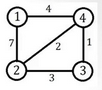
\includegraphics{Kruskal/Grafo4.png}
            \caption{Gráfo de 4 nodos y 5 arcos}
            \label{Grafo4}
        \end{figure}
            
        El archivo que describe la estructura del grafo es:
        \begin{figure}[h!]
            \centering
            \begin{verbatim}
                1{2$7,4$4}
                2{1$7,3$3,4$2}
                3{2$3,4$1}
                4{1$4,2$2,3$1} \end{verbatim}
            \caption{Estructura del grafo \ref{Grafo4} en el archivo}
            \label{ArchivoGrafo4}
        \end{figure} 
        
        Y el árbol mínimo recorrido encontrado fue: \textbf{F\$7=\{ (3,4)  (2,4)  (1,4) \}}
        
        \subsubsection*{Grafo de 5 nodos}
        Grafo de únicamente 5 nodos. Fig\ref{Grafo5} y su estructura en \ref{ArchivoGrafo5}.
        
        \begin{figure}[h!]
            \centering
            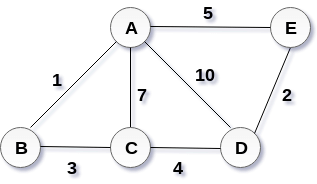
\includegraphics[width=6cm]{Kruskal/Grafo5.png}
            \caption{Gráfo de 5 nodos y 7 arcos}
            \label{Grafo5}
        \end{figure}
            
        El archivo que describe la estructura del grafo es:
        \begin{figure}[h!]
            \centering
            \begin{verbatim}
                A{B$1,C$7,D$10,E$5}
                B{A$1,C$3}
                C{A$7,B$3,D$4}
                D{A$10,C$4,E$2}
                E{A$5,D$2}\end{verbatim}
            \caption{Estructura del grafo \ref{Grafo5} en el archivo}
            \label{ArchivoGrafo5}
        \end{figure} 
        
        Y el árbol mínimo recorrido encontrado fue: \textbf{F\$11=\{ (A,B)  (D,E)  (B,C)  (A,E) \}}
        
        \subsubsection*{Grafo de 6 nodos}
        Grafo de 6 nodos. Fig\ref{Grafo6} y su estructura en \ref{ArchivoGrafo6}.
        
        \begin{figure}[h!]
            \centering
            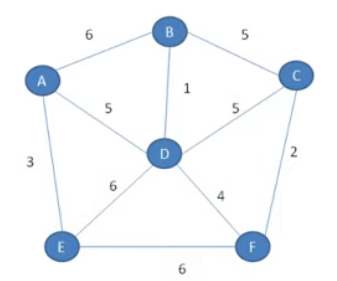
\includegraphics[width=6cm]{Kruskal/Grafo6.png}
            \caption{Gráfo de 6 nodos y 10 arcos}
            \label{Grafo6}
        \end{figure}
            
        El archivo que describe la estructura del grafo es:
        \begin{figure}[h!]
            \centering
            \begin{verbatim}
                A{B$6,D$5,E$3}
                B{A$6,C$5,D$1}
                C{B$5,D$5,F$2}
                D{A$5,B$1,C$5}
                E{A$3,D$6,F$6}
                F{C$2,D$4,E$6}\end{verbatim}
            \caption{Estructura del grafo \ref{Grafo6} en el archivo}
            \label{ArchivoGrafo6}
        \end{figure} 
        
        Y el árbol mínimo recorrido encontrado fue: \textbf{F\$15=\{ (B,D)  (C,F)  (A,E)  (F,D)  (A,D) \}}
        
        \subsubsection*{Grafo de 7 nodos}
        Grafo de 7 nodos. Fig\ref{Grafo7} y su estructura en \ref{ArchivoGrafo7}.
        
        \begin{figure}[h!]
            \centering
            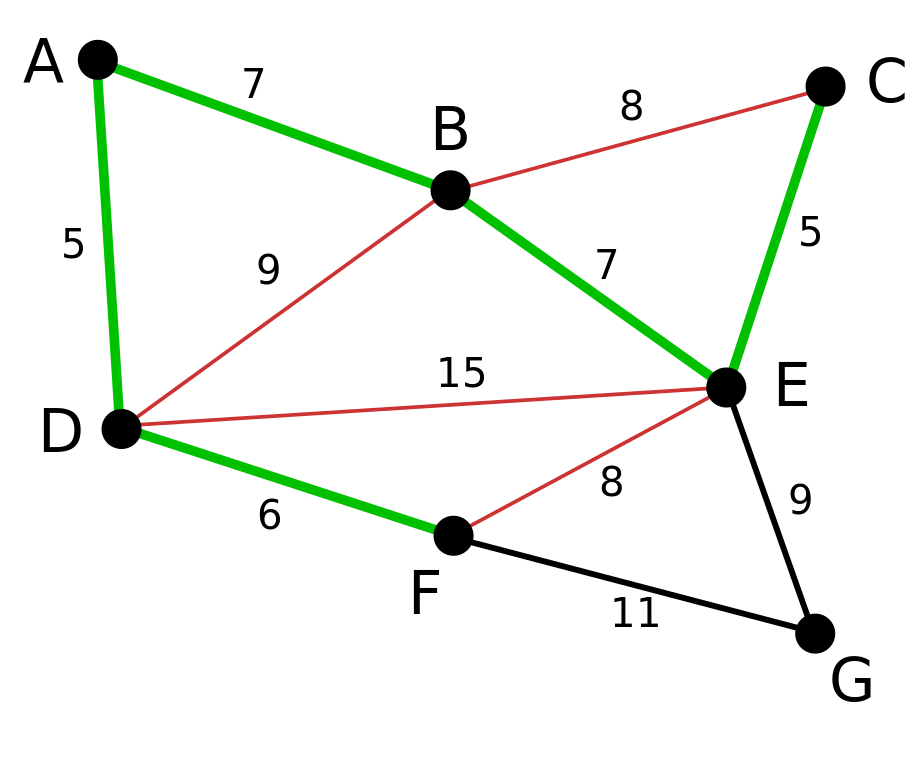
\includegraphics[width=6cm]{Kruskal/Grafo7.png}
            \caption{Gráfo de 7 nodos y 11 arcos}
            \label{Grafo7}
        \end{figure}
            
        El archivo que describe la estructura del grafo es:
        \begin{figure}[h!]
            \centering
            \begin{verbatim}
            A{B$7,D$5}
            B{A$7,C$8,D$9,E$7}
            C{B$8,E$5}
            D{A$5,B$9,E$15,F$6}
            E{B$7,C$5,D$15,F$8,G$9}
            F{D$6,E$8,G$11}
            G{E$9,F$11}\end{verbatim}
            \caption{Estructura del grafo \ref{Grafo7} en el archivo}
            \label{ArchivoGrafo7}
        \end{figure} 
        
        Y el árbol mínimo recorrido encontrado fue: \textbf{F\$41=\{ (C,E)  (A,D)  (D,F)  (B,E)  (E,G)  (B,D) \}}
    
        \newpage
    
        \subsubsection*{Grafo de 8 nodos}
        Grafo de 8 nodos. Fig\ref{Grafo8} y su estructura en \ref{ArchivoGrafo8}.
        
        \begin{figure}[h!]
            \centering
            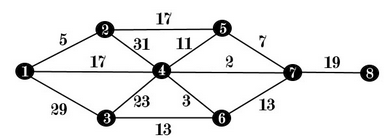
\includegraphics[width=6cm]{Kruskal/Grafo8.png}
            \caption{Gráfo de 8 nodos y 13 arcos}
            \label{Grafo8}
        \end{figure}
            
        El archivo que describe la estructura del grafo es:
        \begin{figure}[h!]
            \centering
            \begin{verbatim}
            1{2$5,3$29,4$17}
            2{1$5,4$31,5$17}
            3{1$29,4$23,6$13}
            4{1$17,2$31,3$23,5$11,6$3,7$2}
            5{2$17,4$11,7$7}
            6{3$13,4$3,7$13}
            7{4$2,5$7,6$13,8$19}
            8{7$19}\end{verbatim}
            \caption{Estructura del grafo \ref{Grafo8} en el archivo}
            \label{ArchivoGrafo8}
        \end{figure} 
        
        Y el árbol mínimo recorrido encontrado fue: \textbf{F\$64=\{ (4,7)  (4,6)  (1,2)  (5,7)  (3,6)  (2,5)  (1,4) \}}

    \newpage

        \subsubsection*{Grafo de 9 nodos}
        Grafo de 9 nodos. Fig\ref{Grafo9} y su estructura en \ref{ArchivoGrafo9}.
        
        \begin{figure}[h!]
            \centering
            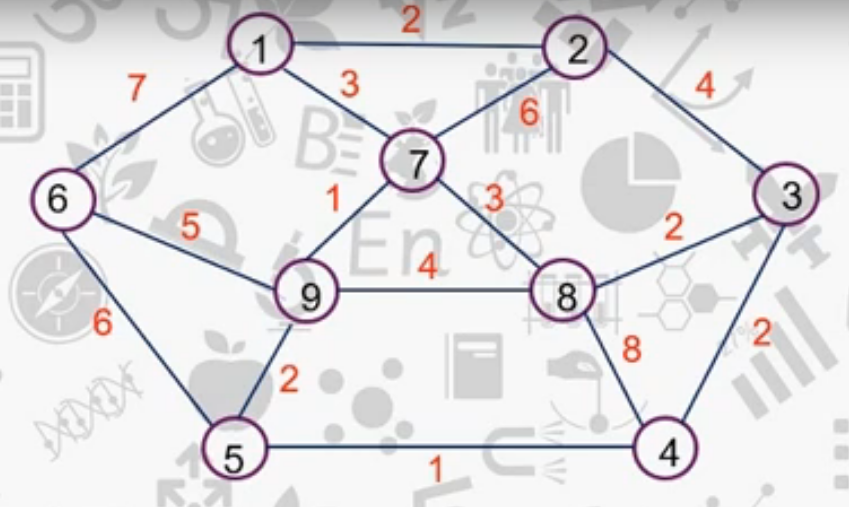
\includegraphics[width=6cm]{Kruskal/Grafo9.png}
            \caption{Gráfo de 9 nodos y 15 arcos}
            \label{Grafo9}
        \end{figure}
            
        El archivo que describe la estructura del grafo es:
        \begin{figure}[h!]
            \centering
            \begin{verbatim}
            1{2$2,7$3,6$7}
            2{1$2,7$6,3$4}
            3{2$4,8$2,4$2}
            4{3$2,8$8,5$1}
            5{4$1,9$2,6$6}
            6{5$6,9$5,1$7}
            7{1$3,2$6,8$3,9$1}
            8{3$2,4$8,9$4,7$3}
            9{7$1,8$4,5$2,6$5}\end{verbatim}
            \caption{Estructura del grafo \ref{Grafo9} en el archivo}
            \label{ArchivoGrafo9}
        \end{figure} 
        
        Y el árbol mínimo recorrido encontrado fue: \textbf{F\$18=\{ (7,9)  (4,5)  (5,9)  (3,4)  (3,8)  (1,2)  (1,7)  (6,9) \}}
    
    \newpage
    
        \subsubsection*{Grafo de 10 nodos}
        Grafo de 10 nodos. Fig\ref{Grafo10} y su estructura en \ref{ArchivoGrafo10}.
        
        \begin{figure}[h!]
            \centering
            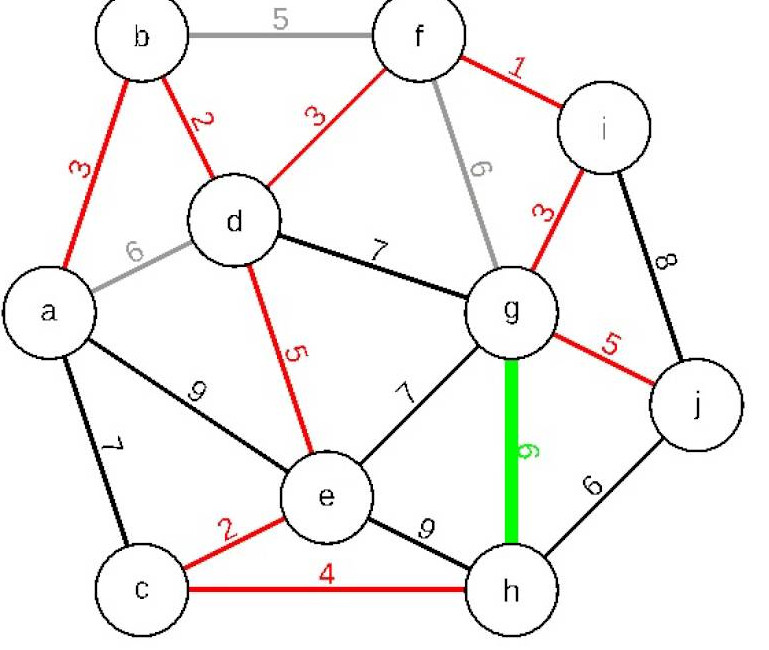
\includegraphics[width=6cm]{Kruskal/Grafo10.jpeg}
            \caption{Gráfo de 10 nodos y 15 arcos}
            \label{Grafo10}
        \end{figure}
            
        El archivo que describe la estructura del grafo es:
        \begin{figure}[h!]
            \centering
            \begin{verbatim}
            a{b$3,d$6,e$9,c$7}
            b{a$3,d$2,f$5}
            c{a$7,e$2,h$4}
            d{a$6,b$2,e$5,f$3,g$7}
            e{a$9,c$2,d$5,g$7,h$9}
            f{b$5,d$3,g$6,i$1}
            g{d$7,e$7,f$6,h$6,i$3,j$5}
            h{c$4,e$9,g$6,j$6}
            i{f$1,g$3,j$8}
            j{g$5,h$6,i$8}\end{verbatim}
            \caption{Estructura del grafo \ref{Grafo10} en el archivo}
            \label{ArchivoGrafo10}
        \end{figure} 
        
        Y el árbol mínimo recorrido encontrado fue: \textbf{F\$28=\{ (f,i)  (c,e)  (b,d)  (g,i)  (d,f)  (a,b)  (c,h)  (g,j)  (b,f) \}}
        
        \newpage
        
        \subsubsection{Propuesta de complejidad}
        A partir de estos 8 archivos ingresados y evaluados por el programa, la gráfica en la figura \ref{GraficaKruskal} muestra el resultado de la comparación del número de nodos o aristas del grafo ingresado, contra el número de operaciones realizadas para cada archivo:
        \begin{figure}[h!]
            \centering
            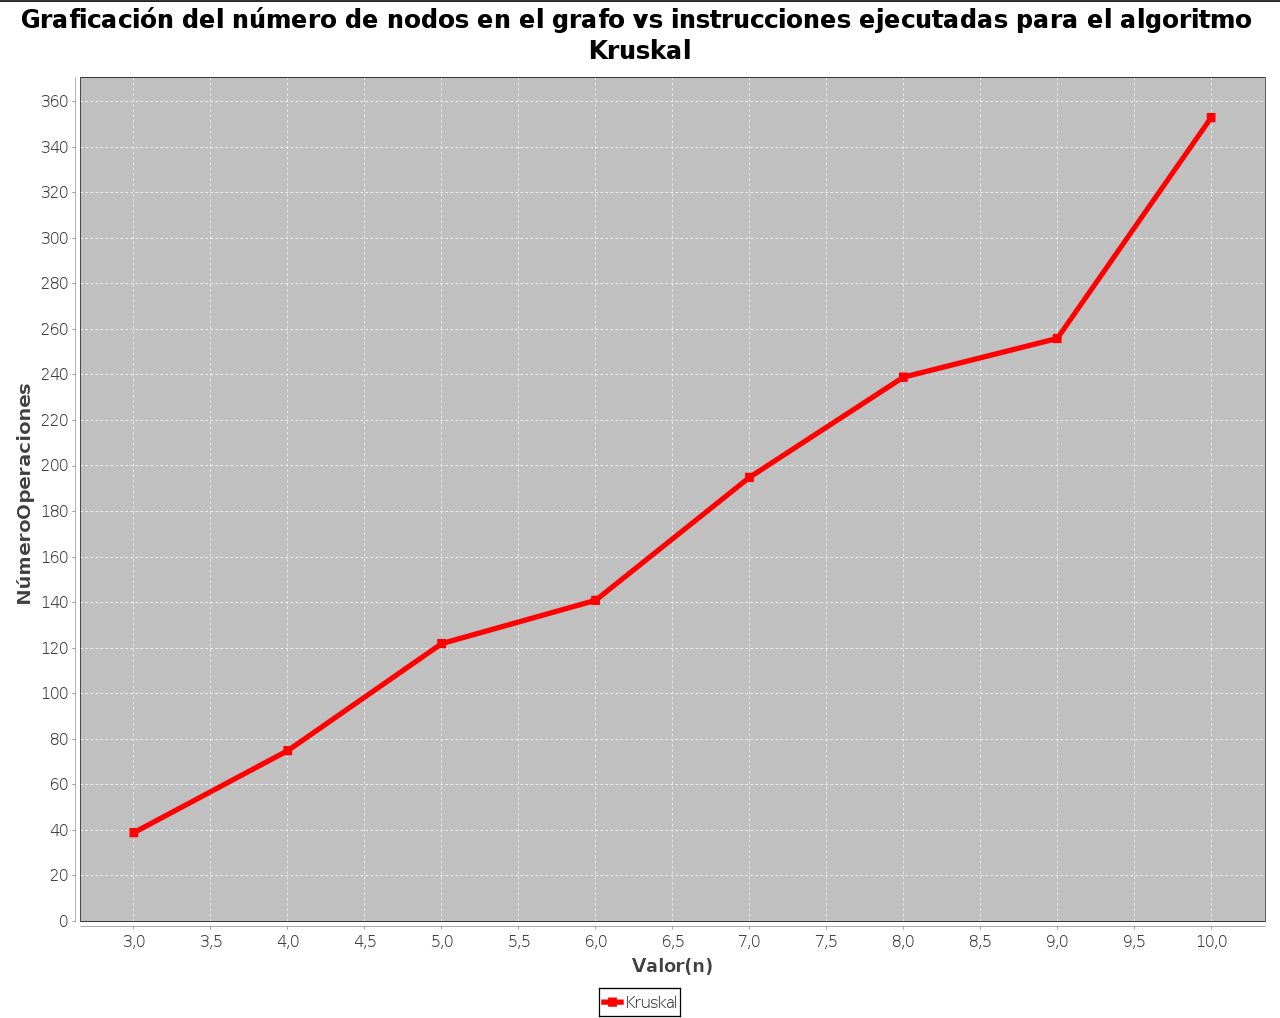
\includegraphics[width=16cm]{Kruskal/GraficaKruskal.png}
            \caption{Gráfica generada a partir de la evaluación de los archivos con los grafos descritos\\ En el eje de las abcisas se encuentra el número de nodos del grafo y en el de las ordenadas el número de operaciones realizadas}
            \label{GraficaKruskal}
        \end{figure}
        Y los puntos que genera esta gráfica son \ref{PuntosKruskal}:
        \begin{figure}[h!]
            \centering
            \begin{tabular}{c c}
                P1( 3 ,39 ) & P5( 7 ,195 ) \\
                P2( 4 ,75 ) & P6( 8 ,239 )\\
                P3( 5 ,122 ) & P7( 9 ,256 )\\
                P4( 6 ,141 ) & P8( 10 ,353 )\\
            \end{tabular}
            \caption{Puntos obtenidos de la evaluacion de los 8 grafos especificados anteriormente}
            \label{PuntosKruskal}
        \end{figure}
        
        Y es con estos datos obtenidos que se propone la complejidad para este algoritmo. En la figura \ref{GraficaComplejidadKruskal} se muestran los puntos obtenidos y 2 ecuaciones que acotan a estos mismos. Es evidente desde la figura \ref{GraficaKruskal} que su cota superior no podría ser lineal pues el crecimiento que experimenta en el eje de las ordenadas es muy veloz en comparación con una complejidad lineal.\\
        
        \begin{figure}[h!]
            \centering
            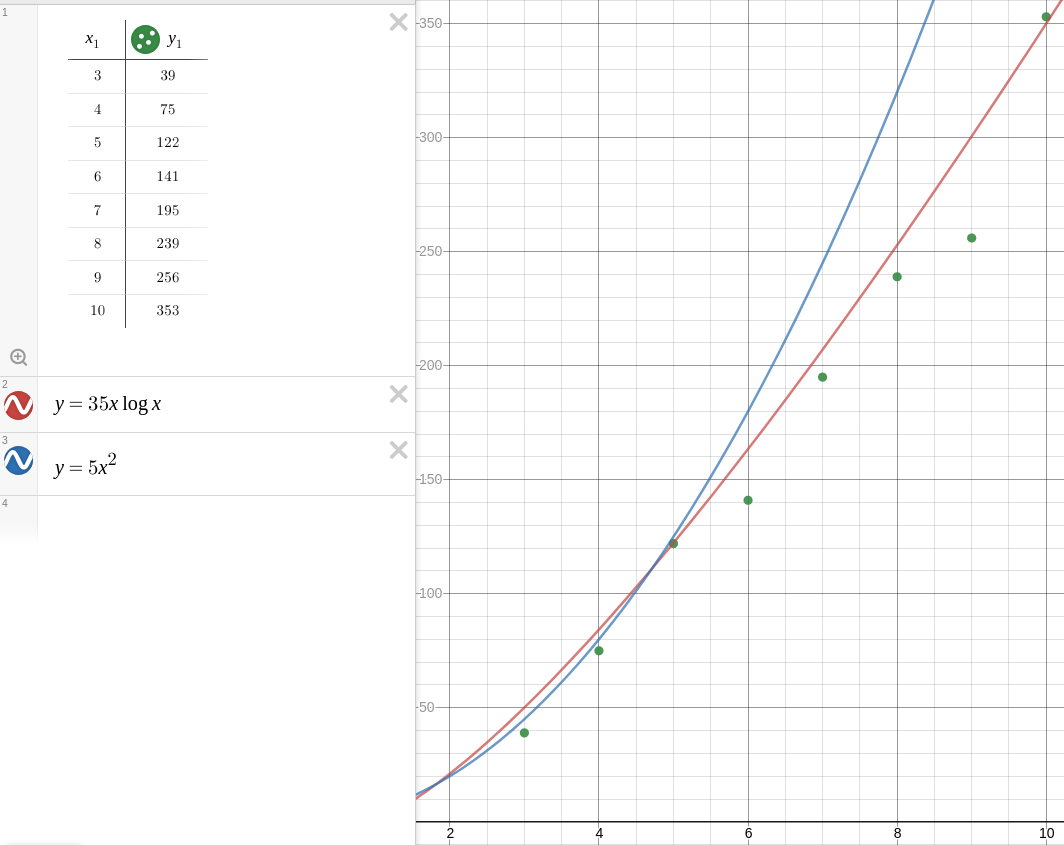
\includegraphics[width=19cm]{Kruskal/GraficaComplejidadKruskal.png}
            \caption{Gráfica de la proposición para la complejidad para el algoritmo de Kruskal\\ Los puntos verdes corresponden a los puntos obtenidos de la evaluación de los grafos \\ La curva de color rojo corresponde a la cota de orden \textit{n logn}\\ La curva de color azul corresponde a la cota de orden $n^2$}
            \label{fig:my_label}
        \end{figure}
        
        Por esta razón se propone hacer una comparación de las 2 cotas siguientes superiores, la cota \textit{nlogn} y $n^2$.\\
        
        Mediante la asignación arbitraria de valores constantes que multiplican a los términos, observamos claramente que una cota del orden \textit{nlogn}, se ajusta de forma más justa y describiendo un comportamiento parecido al de los puntos.\\
        
        Mientras que la cota cuadrática en un principio parece acotar de forma más justa a los primeros 3 puntos, su crecimiento será muy superior con los datos obtenidos posteriores.\\
        
        De tal manera que se afirma que para el algoritmo de Kruskal que permite encontrar un árbol mínimo recubridor en un grafo conexo no dirigido y ponderado será:
        \begin{equation*}
            \text{\textbf{kruskal(n)}}\in\text{\textbf{O(n log n)}}
        \end{equation*}

\subsection*{Investigación complejidad}

    Los elementos escenciales para el funcionamiento del algoritmo, y por consiguiente los que nos darán el tiempo de ejecución, serán en general el grafo, pero siendo más especificos, los elementos que componen al arbol. Las aristas(\textbf{a}) y los vértices(\textbf{v}), que ya se especificó antes se encuentran ponderados mediante un costo, son los 2 elementos principales que intervienen en la complejidad del algoritmo.\\
    
    Se considera que para el algoritmo de Kruskal la complejidad será a lo más \textbf{O(a log a)}, siendo equivalente la cota \textbf{O(a log n)}, cuando los datos se encuentran almacenados mediante estructuras simples.\\
    
    La razón por la que estas 2 cotas son equivalentes se debe a:
    \begin{itemize}
        \item Las aristas serán a los más $v^2$, y el $logv^2 = 2logv$ que puede calcularse mediante diversos métodos, pero otorga una complejidad de \textbf{O(log v)}
        \item Se ignoran los vértices aislados, esto debido que forman su propia componente del árbol de expansión mínimo, los vertices son menores o iguales a el doble de las aristas $v\leq 2a$, resultando entonces que el logn es \textbf{O(loga)}
    \end{itemize}
    
    Para poder conseguir esta complejidad es primordial ordenar las aristas en función del peso, mediante un algoritmo con complejidad \textit{O(a log a)}, como lo es \textit{Comparison sort}. Esta ordenación permite que la eliminación de una arista con peso mínimo pueda ejecutarse en un tiempo constante.\\
    
    Ahora, dado que es necesario el control de los vértices para identificar cuales de estos están en que componentes, se utiliza una estructura de datos sobre conjuntos disjuntos. La complejidad del ordenamiento de este será \textit{O(a)} operaciones, esto se debe a 2 operaciones de búsqueda por arista, y una posible unión de conjuntos.\\
    
    Finalmente se considera que inclusive con una estructura de conjuntos disjuntos simples con uniones poir rangos, es capaz de ejecutar las operaciones mencionadas en un tiempo \textbf{O(a log v)}, se considera que el orden de este algoritmo es:
    \begin{equation*}
        \text{\textbf{O(a log a) = O(a log v)}}
    \end{equation*}
    
    Este algoritmo permite además encontrar soluciones para estructuras de conjuntos disjuntos complejos, tales como los bosques, es posible acotar los tiempos de ejecución en \textbf{O(a $\alpha$(v))}, de donde $\alpha$ es la inversa de la \textit{Función de Ackermann}.\\
    
    La función de \textit{Ackermann}, es un función matemática recursiva que fue encontrada en el año de 1926 por el matemático alemán Willhelm Ackermann. Que tienen cono particularidad, un crecimiento extremadamente rápido, lo que consecuentemente las volvería un recurso interesante para la ciencia computacional teórica y la teoría de computabilidad.\\
    
    Es precisamente por esta característica, que el valor de su inversa tendrá el comportamiento contrario, un crecimiento sumamente lento, dotando de una complejidad aún muy controlada inclusive cuando se trabaja con estructuras complejas para el algoritmo de Kruskal.
        \newpage
        
\chapter*{Conclusiones}
    \begin{tabular}{l l}
        \multirow{3}{*}{
\includegraphics[width=1.5cm]{Imagenes/imanol.jpg}} &  \\
        & \textbf{Rivero Ronquillo Omar Imanol}\\
        & \\
    \end{tabular}
    \vspace*{3\baselineskip}\\
    Nunca había pensado en las formas en las que se podría optimizar la solución a un problema por medio de un algoritmo programable. Me pareció un enfoque increíble y ahora me parece que tengo claro porque se usan estos algorimos y en qué problemas se les podría dar un uso. A pesar de que en comparación con las prácticas anteriores se tuvieron que incluir más cosas además de los algorimos, para poder probarlos y estudiarlos, me parecieron un gran complemento en mi formación académica.
    
    En conclusión, me gustaría conocer más algoritmos de este tipo, me interesaron especialmente los algoritmos de compresión, aunque puedo estar bastante seguro de que las compresiones modernas deberán de tener una complejidad mayor de aprenderse y comprender su funcionamiento, que seguramente justificaran todo esto con las tasas de compresiones que puedan lograr.
    \\\\
    \begin{tabular}{l l}
        \multirow{3}{*}{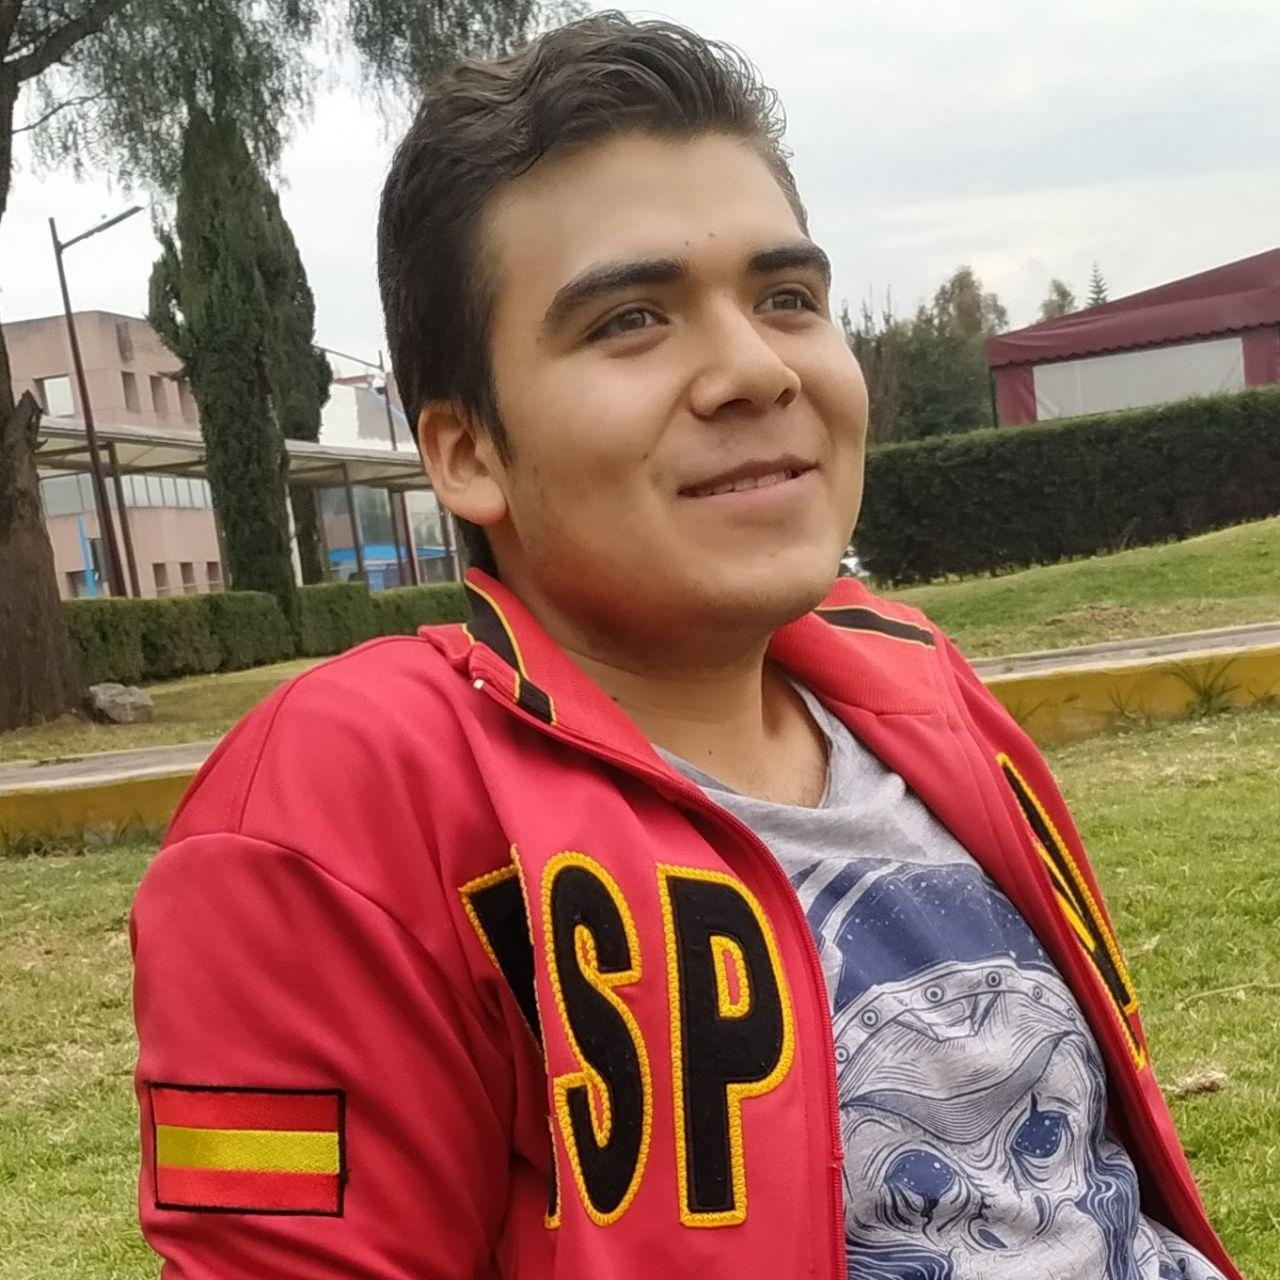
\includegraphics[width=1.5cm]{Imagenes/lalo.jpg}}  &  \\
        & \textbf{Valle Mart\'inez Luis Eduardo} \\
        & \\
    \end{tabular}
    \vspace*{3\baselineskip}\\
    

\end{document}
